\documentclass{article}
\usepackage{amsmath}
\usepackage{amssymb}
\usepackage{graphicx}
\usepackage{hyperref}
\usepackage[version=4]{mhchem}

\title{Example 9}
\date{}

\begin{document}
\maketitle

(AMC) Distinct points \(A\) and \(B\) are on a semicircle with diameter \(M N\) and center \(C\). The point \(P\) is on \(C N\) and \(\angle C A P=\angle C B P=10^{\circ}\). If \(\wideparen{M A}=40^{\circ}\), then \(\wideparen{B N}\) equals\\
(A) \(10^{\circ}\)\\
(B) \(15^{\circ}\)\\
(C) \(20^{\circ}\)\\
(D) \(25^{\circ}\)\\
(E) \(30^{\circ}\)

Solution: (C).\\
\centering
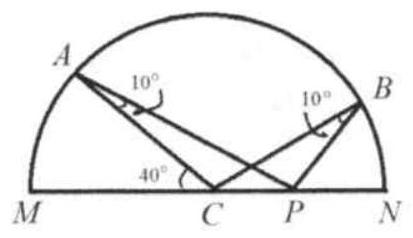
\includegraphics[width=\textwidth]{images/problem_image_1.jpg}

Method 1:\\
In \(\triangle A C P\) and \(\triangle B C P\) we have (in the order given) the condition angle-side-side.\\
Since these triangles are not congruent \((\angle C P A \neq \angle C P B)\), we must have that \(\angle C P A\) and \(\angle C P B\) are supplementary.\\
From \(\triangle A C P\) we compute\\
\(\angle C P A=180^{\circ}-10^{\circ}-\left(180^{\circ}-40^{\circ}\right)=30^{\circ}\).\\
Thus \(\angle C P B=150^{\circ}\) and \(\wideparen{B N}=\angle P C B=180^{\circ}-10^{\circ}-150^{\circ}=20^{\circ}\).


Method 2:
\(\angle C P A=30^{\circ}(\operatorname{arc} A C)\)\\
\(\angle C B A=30^{\circ}(\operatorname{arc} A C)\)\\
\(\angle C A B=\angle C B A(\operatorname{arc} B C=\operatorname{arc} A C)\)\\
\(\angle P A B=30^{\circ}-10^{\circ}=20^{\circ}\).\\
\(\angle B C P=\angle P A B=20^{\circ}\) (same arc \(P B\) ).\\
\centering
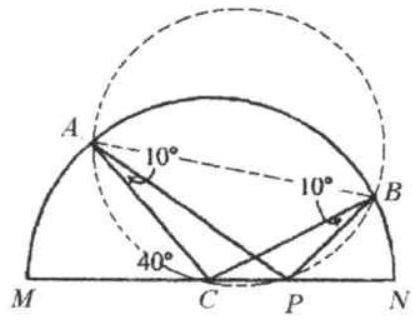
\includegraphics[width=\textwidth]{images/reasoning_image_1.jpg}


\end{document}
